\documentclass{article}
\usepackage[utf8]{inputenc}
\usepackage[margin=1in]{geometry}
\usepackage{soul,color}
\usepackage{amsfonts, amsmath}
\usepackage{bbm}
\usepackage{enumitem}
\usepackage[nobreak=true]{mdframed}
\usepackage{graphicx}

\newcommand{\solution}{\textbf{Solution: }}
\newcommand{\N}{\mathcal{N}}
% \newcommand{\Pbf}{\textbf{P}}
\newcommand{\R}{\mathbb{R}}
\newcommand{\E}{\mathbb{E}}
\newcommand{\Var}{\text{Var}}
\newcommand{\Cov}{\text{Cov}}


% Default fixed font does not support bold face
\DeclareFixedFont{\ttb}{T1}{txtt}{bx}{n}{8} % for bold
\DeclareFixedFont{\ttm}{T1}{txtt}{m}{n}{8}  % for normal

% Custom colors
\usepackage{color}
\definecolor{deepblue}{rgb}{0,0,0.5}
\definecolor{deepred}{rgb}{0.6,0,0}
\definecolor{deepgreen}{rgb}{0,0.5,0}

\usepackage{listings}

% Python style for highlighting
\newcommand\pythonstyle{\lstset{
language=Python,
basicstyle=\ttfamily\footnotesize,
otherkeywords={self},             % Add keywords here
keywordstyle=\ttb\color{deepblue},
emph={MyClass,__init__},          % Custom highlighting
emphstyle=\ttb\color{deepred},    % Custom highlighting style
stringstyle=\color{deepgreen},
frame=tb,                         % Any extra options here
showstringspaces=false           % 
}}


% Python environment
\lstnewenvironment{python}[1][]
{
\pythonstyle
\lstset{#1}
}
{}

% Python for external files
\newcommand\pythonexternal[2][]{{
\pythonstyle
\lstinputlisting[#1]{#2}}}

% Python for inline
\newcommand\pythoninline[1]{{\pythonstyle\lstinline!#1!}}

\title{CS189, HW6: Neural Nets}
\author{ Completed by: Matthew Wu}
% \date{January 2017}
\date{}

\begin{document}

\maketitle

\subsection*{Problem 1: Derivations}

Let $X$ be the matrix of sample points.\\
Let $X^1$ be the matrix of sample points with a column of a bias dimension augmented to the end.\\
Let $x$ be a row of $X$ (784 dimensions), and let $x^1$ be a row of $X_1$ (785 dimensions).\\
Similarly, let $h$ be the hidden units (200 dimensions), and let $h^1$ be the hidden units with a bias unit appended to the end (201 dimensions).\\
Let $z$ be the 26 dimension output layer.\\
\\
Let $V$ be the $200 \times 784$ matrix for the weights between $x$ and $h$ (without bias).\\
Let $V^1$ be the $200 \times 785$ matrix for the weights between $x_1$ and $h$ (with bias).\\
Let $W$ be the $26 \times 200$ matrix for the weights between $h$ and $z$ (without bias).\\
Let $W^1$ be the $26 \times 201$ matrix for the weights between $h_1$ and $z$ (with bias).\\
\\
Let $y$ be the desired output (26 dimensions).\\
Let $\mathbbm{1}$ denote a vector of ones, and $\circ$ be the Hadamard product.

$$\tanh(V^1x^1)=h$$
$$s(W^1h^1)=z$$
$$L(z, y) = -\sum_{j=1}^{26}y_jln(z_j) + (1-y_j)ln(1-z_j)$$
$$\frac{\partial L}{\partial z_j} -\frac{y_j}{z_j}+\frac{1-y_j}{1-z_j}=\frac{z_j-y_j}{z_j(1-z_j)}$$
$$\nabla_{W^1_j}L=\frac{\partial L}{\partial z_j}\nabla_{W^1_j}z_j=\frac{\partial L}{\partial z_j} z_j(1-z_j)h^1=(z_j-y_j)h^1 \Rightarrow \nabla_{W^1}L=(z-y){h^1}^T$$
$$\nabla_hL = \sum_{j=1}^k \frac{\partial L}{\partial z_j}\nabla_hz_j=\sum_{j=1}^{26}z_j(1-z_j)\frac{\partial L}{\partial z_j}W_j = \sum_{j=1}^{26}(z_j-y_j)W_j=W^T(z-y)$$
$$h_i=\tanh(V^1_ix^1_i)\Rightarrow \nabla_{V^1_i}h^1_i=\tanh'(V^1_i \cdot x)x=(1-{h^1_i}^2)x$$
$$\nabla_{V^1_i}L=\frac{\partial L}{\partial h_i}\nabla_{V^1_i}h_i=\frac{\partial L}{\partial h_i}(1-{h^1_i}^2)x^1 \Rightarrow \nabla_{V^1}L=((\mathbbm{1}-h \circ h) \circ \nabla_hL){x^1}^T$$

Suppose that we pick a learning rate of $\epsilon$. Then our updates for $V^1$ and $W^1$ will be:

$$V^1 \leftarrow V^1 - \epsilon((\mathbbm{1}-h \circ h) \circ W^T(z-y)){x^1}^T$$
$$W^1 \leftarrow W^1 - \epsilon(z-y){h^1}^T$$

\newpage
\subsection*{Problem 2: Implementation}    
\begin{enumerate}
    \item Any hyperparameters that you tuned.
    \begin{mdframed}
    \solution The only hyper-parameter I ended up tuning was epsilon. Trial and error led to the conclusion that a value of $\epsilon = .002$ worked.
    \end{mdframed}
        
    \item Your training accuracy.
    \begin{mdframed}
    \solution Training accuracy is about .88336 after 5 epochs.
    \end{mdframed}
        
    \item Your validation accuracy.
    \begin{mdframed}
    \solution Validation accuracy is about .86142 after 5 epochs.
    \end{mdframed}
        
    \item A plot of the loss value versus the number of iterations. You may sample (i.e., compute the loss every $x$ iterations).
    \begin{mdframed}
    \solution
    
    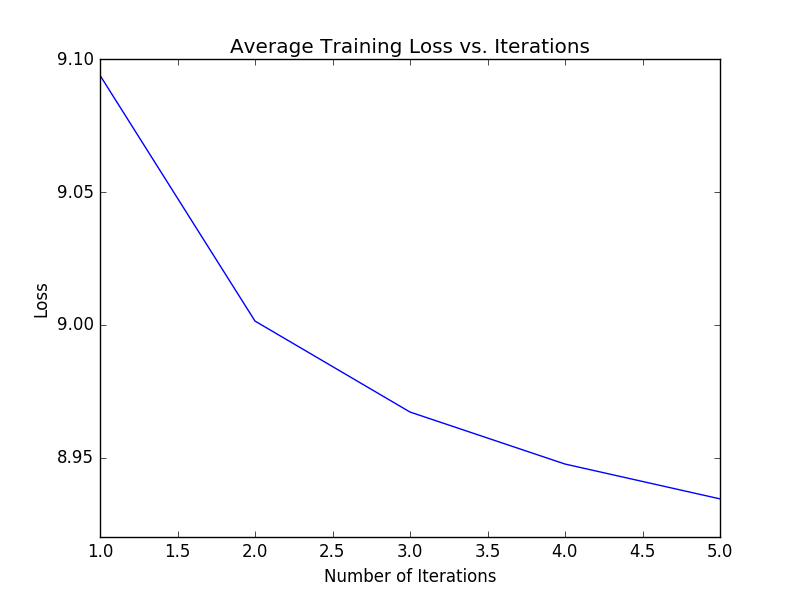
\includegraphics[scale=.6]{loss.png}\\
    \end{mdframed}
    \item Your Kaggle score and display name.
    \begin{mdframed}
    \solution
    
    Name: Commendable Fennel
    
    Score: .85692
    \end{mdframed}
        
    \item Your code (as an appendix at the end).
\end{enumerate}

\noindent   
Expect validation accuracies of 85\% or higher. Your TAs are able to achieve 87.3\% validation accuracy after 1 minute of training on a MacBook Pro. With some tweaks (800 hidden units, ReLU hidden layer activation, softmax output layer activation), your TAs are able to get 90.17\% validation accuracy after 3 minutes of training.

\newpage
\subsection*{Problem 3: Visualization}
Correctly classified images:\\

\includegraphics[scale=1]{right0.png} S\\

\includegraphics[scale=1]{right1.png} L\\

\includegraphics[scale=1]{right2.png} B\\

\includegraphics[scale=1]{right3.png} I\\

\includegraphics[scale=1]{right4.png} X\\

Incorrectly classified images:\\

\includegraphics[scale=1]{wrong0.png} Classified as B instead of D\\

\includegraphics[scale=1]{wrong1.png} Classified as R instead of Y\\

\includegraphics[scale=1]{wrong2.png} Classified as U instead of D\\

\includegraphics[scale=1]{wrong3.png} Classified as L instead of I\\

\includegraphics[scale=1]{wrong4.png} Classified as L instead of I\\

\newpage
\subsection*{Problem 4: Bells and Whistles}
In lecture, we covered many variations and ways to improve the learning speed and accuracy of neural networks. After you have implemented the basic neural network as we have prescribed, you may go above and beyond to improve your network for your Kaggle submissions. As with Problem 2, you must implement any additional functionality yourself. (E.g., you \textbf{cannot} train a neural network with Tensorflow and use that.) In this section of your writeup, report any extra functionality or tricks you implemented. Some ideas:
    
\begin{itemize}
    \item Use different learning rates for different layers, and have those rates decay over time. (Highly recommended. See Section 5.4.)
    \item Change the number of hidden layer units, or even add one or more additional hidden layers.
    \item Use different activation functions. ReLUs for the hidden layer and softmax output units can speed up training and improve accuracy.
    \item Implement mini-batch gradient descent. This will dramatically speed up your training time.
    \item Regularization: both $L_2$ regularization and dropout are surprisingly easy to implement, and tend to reduce overfitting.
    \item Momentum, different initialization schemes, an ensemble of neural networks, etc. See the “Implementation Tips” section for ideas.
\end{itemize}
    
\begin{mdframed}
\solution I implemented mini-batch gradient descent using 40 sample points at a time to speed up training time.
\end{mdframed}

\newpage

\subsection*{Appendix}
The following code was used for everything:

\begin{python}
import numpy as np
import scipy.io
import matplotlib.pyplot as plt
import csv
import scipy.misc
import sys

traindatafilename = "hw6_data_dist/letters_data"
data = scipy.io.loadmat(traindatafilename)

TRAINING_FRACTION = .8

traindata = data['train_x']
trainlabels = data['train_y']

NUM_FEATURES = traindata.shape[1]
NUM_SAMPLES = traindata.shape[0]

testdata = data['test_x']

#Shuffle the training data
temp = np.hstack((traindata, trainlabels))
np.random.shuffle(temp)
X = temp[:,:NUM_FEATURES]
y = temp[:,NUM_FEATURES:]

#Add bias terms and normalize all data
"""
temp = np.vstack((X, testdata))
temp = np.hstack((temp, np.ones(temp.shape[0]).reshape(temp.shape[0], 1)))
temp = temp / (np.linalg.norm(temp, axis=0)[np.newaxis, :] + .000000001)
temp = temp - np.mean(temp, axis=0)
X = temp[:NUM_SAMPLES]
testdata = temp[NUM_SAMPLES:]
"""

column_means = np.mean(X, axis=0)

X = X - column_means
testdata = testdata - column_means

column_stds = np.std(X, axis=0) + .000000001
X = X / column_stds
testdata = testdata / column_stds

X = np.hstack((X, np.ones(X.shape[0]).reshape(X.shape[0], 1)))
testdata = np.hstack((testdata, np.ones(testdata.shape[0]).reshape(testdata.shape[0], 1)))

#Increment features by 1 to account for bias
NUM_FEATURES += 1

#Create training and validation sets
TRAINING_SIZE = int(TRAINING_FRACTION * NUM_SAMPLES)
VALIDATION_SIZE = NUM_SAMPLES - TRAINING_SIZE
sys.stdout.flush()

X_train = X[:TRAINING_SIZE]
y_train = y[:TRAINING_SIZE]

X_validation = X[TRAINING_SIZE:]
y_validation = y[TRAINING_SIZE:]

#END PREPROCESSING DATA

#Initialize constants and matrices
EPSILON = .002
decay_factor = .85
V = np.random.normal(0, .01, (200, 785))
W = np.random.normal(0, .01, (26, 201))

y_array = [None]
for i in range(26):
    temp = np.ones((26, 1)) * .1
    temp[i] = .9
    y_array.append(temp)

def sigmoid(num):
    return 1 / (1 + np.exp(-num))

def classify(sample):
    h = np.tanh(np.dot(V, sample)).reshape((200, 1))
    h1 = np.vstack((h, 1))
    z = sigmoid(np.dot(W, h1))
    return np.argmax(z) + 1

def caclulate_validation_accuracy():
    right = 0
    for i in range(VALIDATION_SIZE):
        sample = X_validation[i]
        guess = classify(sample)
        label = y_validation[i]
        if guess == label:
            right += 1
    return right / VALIDATION_SIZE

def calculate_training_accuracy():
    right = 0
    for i in range(TRAINING_SIZE):
        sample = X_train[i]
        guess = classify(sample)
        label = y_train[i]
        if guess == label:
            right += 1
    return right / TRAINING_SIZE

def calculate_training_loss():
    total_loss = 0
    for i in range(TRAINING_SIZE):
        x = X_train[i]
        h = np.tanh(np.dot(V, x).reshape((200, 1)))
        h1 = np.vstack((h, 1))
        z = sigmoid(np.dot(W, h1))
        y = y_array[int(y_train[i])]
        total_loss += loss(z, y)
    return float(total_loss / TRAINING_SIZE)

def loss(z, y):
    l = 0
    for i in range(26):
        zi, yi = z[i], y[i]
        l -= yi*np.log(zi) + (1-yi)*np.log(1-zi)
    return l

def plot_loss(loss_array):
    iterations = [i + 1 for i in range(len(loss_array))]
    plt.figure()
    plt.plot(iterations, loss_array)
    plt.title("Average Training Loss vs. Iterations")
    plt.ylabel("Loss")
    plt.xlabel("Number of Iterations")
    plt.show()

def save_classified_images():
    right = 0
    wrong = 0
    index = 0
    while right < 5 or wrong < 5:
        sample = X_validation[index]
        guess = classify(sample)
        sample = sample[:784].reshape((28, 28))
        label = y_validation[index]
        if guess == label:
            if right < 5:
                s = 'right' + str(right) + '.png'
                scipy.misc.imsave(s, sample)
                right += 1
                print(s, guess)
        else:
            if wrong < 5:
                s = 'wrong' + str(wrong) + '.png'
                scipy.misc.imsave(s, sample)
                wrong += 1
                print(s, guess, label)
        index += 1

def classify_test_data():
    TEST_SIZE = testdata.shape[0]
    guesses = []
    for i in range(TEST_SIZE):
        sample = testdata[i]
        guesses.append(classify(sample))
    with open('submission_1.csv', 'w', newline='') as csvfile:
        writer = csv.writer(csvfile)
        writer.writerow(['Id', 'Category'])
        i = 1
        for g in guesses:
            writer.writerow([i, g])
            i += 1


loss_array = []
for epoch in range(5):
    for i in range(0, TRAINING_SIZE, 40):
        x = np.transpose(X_train[i:i+40])
        h = np.tanh(np.dot(V, x))
        h1 = np.vstack((h, np.ones(40)))
        z = sigmoid(np.dot(W, h1))
        y = []
        for j in range(40):
            y.append(y_array[int(y_train[i+j])].reshape(26))
        y = np.transpose(y)
        grad_w = np.dot(z-y, np.transpose(h1))
        temp1 = np.ones((200, 40)) - h * h
        temp2 = np.dot(np.transpose(W)[:200], z - y)
        grad_v = np.dot(temp1 * temp2, np.transpose(x))
        V = V - grad_v * EPSILON
        W = W - grad_w * EPSILON
    EPSILON *= decay_factor
    print("Epochs:", epoch + 1)
    training_loss = calculate_training_loss()
    print("Training loss:", training_loss)
    loss_array.append(training_loss)
    sys.stdout.flush()

print("Training accuracy:", calculate_training_accuracy())
print("Validation accuracy:", caclulate_validation_accuracy())

plot_loss(loss_array)
classify_test_data()
save_classified_images()
\end{python}

\end{document}
